% LaTeX path to the root directory of the current project
\providecommand{\econtexRoot}{}
\renewcommand{\econtexRoot}{..}
\providecommand{\econtexPaths}{LaTeX}\renewcommand{\econtexPaths}{\econtexRoot/LaTeX/econtexPaths}
\documentclass[\econtexRoot/BufferStockTheory]{subfiles}
% LaTeX path to the root directory of the current project
\providecommand{\econtexRoot}{}
\renewcommand{\econtexRoot}{..}
\providecommand{\econtexPaths}{LaTeX}\renewcommand{\econtexPaths}{\econtexRoot/LaTeX/econtexPaths}
\input{\LaTeXFiles/onlyinsubfile.sty}

\onlyinsubfile{\externaldocument{\LaTeXFiles/BufferStockTheory}} % Get xrefs -- esp to appendix -- from main file; only works properly if main file has already been compiled;
\begin{document}

  \subsection{Diagrams for the Perfect Foresight Model}
  The diagrams below illustrate the order of the several conditions in the text:
  \providecommand{\tikzFigs}{\econtexRoot/Code/LaTeX}
  \medskip
  
  \centerline{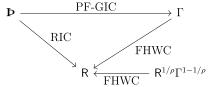
\includegraphics{\tikzFigs/PFGIC-vs-RIC-vs-FHWC}}
% \[
%   \begin{tikzcd}[row sep=large, column sep=large]
%   \textbf{\Thorn} \ar{rr}{\mathrm{\PFGIC}} \ar{dr}{\mathrm{\RIC}}& & \Gamma \ar{dl}{\mathrm{\FHWC}} \\
%    & \mathsf{\Rfree} &
%   \end{tikzcd}
% \]

  and to further incorporate the Perfect Foresight Finite Value of Autarky Condition:
  
  \centerline{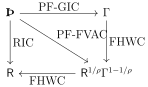
\includegraphics{\tikzFigs/PFGIC-vs-RIC-vs-FHWC-vs-FVAC}}
  
% \[
%   \begin{tikzcd}[row sep=huge, column sep=huge]
%   \textbf{\Thorn} \ar{r}{\mathrm{\PFGIC}} \ar{d}{\mathrm{\RIC}} \ar{dr}{\mathrm{\PFFVAC}}& \Gamma \ar{d}{\mathrm{\FHWC}} \\
%    \mathsf{\Rfree} &  \mathsf{\Rfree}^{1/\CRRA}\Gamma^{1 - 1/\CRRA} \ar{l}{\mathrm{\FHWC}}
%  \end{tikzcd}
%  \]
In both diagrams, an arrow means ``$<$'', which indicates the annotated condition holds, so if a condition is violated, the corresponding arrow is to be reversed. 

These diagrams also keep track of the hierarchy among the conditions. For example, if the right vertical arrow in the second diagram is reversed, then the top right triangle says \PFFVAC + \cncl{\FHWC} implies \PFGIC. If the left vertical arrow is reversed, then \cncl{\RIC} + {\PFGIC} implies \cncl{\FHWC}. 

%\onlyinsubfile{\bibliography{\LaTeXFiles/BufferStockTheory,economics}}


\end{document}
% Local Variables:
% eval: (setq TeX-command-list  (remove '("Biber" "biber %s" TeX-run-Biber nil  (plain-tex-mode latex-mode doctex-mode ams-tex-mode texinfo-mode)  :help "Run Biber") TeX-command-list))
% eval: (setq TeX-command-list  (remove '("Biber" "biber %s" TeX-run-Biber nil  t  :help "Run Biber") TeX-command-list))
% tex-bibtex-command: "bibtex ../LaTeX/*"
% TeX-PDF-mode: t
% TeX-file-line-error: t
% TeX-debug-warnings: t
% LaTeX-command-style: (("" "%(PDF)%(latex) %(file-line-error) %(extraopts) -output-directory=../LaTeX %S%(PDFout)"))
% TeX-source-correlate-mode: t
% TeX-parse-self: t
% eval: (cond ((string-equal system-type "darwin") (progn (setq TeX-view-program-list '(("Skim" "/Applications/Skim.app/Contents/SharedSupport/displayline -b %n ../LaTeX/%o %b"))))))
% TeX-parse-all-errors: t
% End:
